\documentclass[12pt]{article}
\usepackage{preamble}

\pagestyle{fancy}
\fancyhead[LO,LE]{Математический анализ}
\fancyhead[CO,CE]{10.04.2024}
\fancyhead[RO,RE]{Лекции Далевской О. П.}


\begin{document}
    \subsection{5.4. Замена переменной в двойном и тройном интегралах}

    \hypertarget{substitutionindoubleintegral}{}

    Проблема: для $S = \iint_D dxdy$, если $S_{D^\prime} = \int_0^{2\pi} d\varphi \int_0^R d\rho = \iint_{D^\prime} d\rho d\varphi$, то это не площадь круга, а площадь прямоугольника $S$ в распрямленных координатах

    Введем $\Delta s_i$ -- площадь кольцевого сектора в полярных координатах, а $\Delta s^\prime_i$ -- площадь прямоугольника, причем $\Delta s_i \neq \Delta s_i^\prime$

    \Nota Будем искать поправочный коэффициент так, чтобы $\Delta s_i \approx \text{коэфф.} \cdot \Delta s_i^\prime$

    Дроблению будем подвергать область $D^\prime$ в распрямленной системе координат

    Введем новые криволинейные координаты: $\begin{cases}
        x = \varphi(u, v) \\ y = \psi(u, v)
    \end{cases}$,
    где функции $\varphi(u, v), \psi(u, v)$ непрерывно дифференцируемы по обоим аргументам

    \begin{multicols}{2}
        \centering
        % https://www.geogebra.org/calculator/qrgrgvq7
        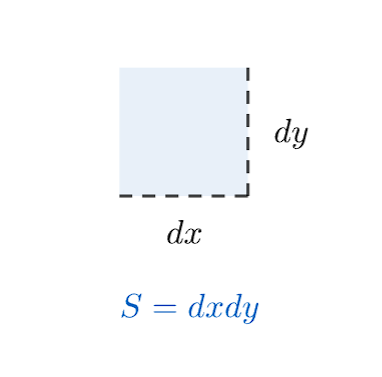
\includegraphics[height=7cm]{calculus/images/calculus_2024_04_10_1}

        % https://www.geogebra.org/calculator/ypbfdhhk
        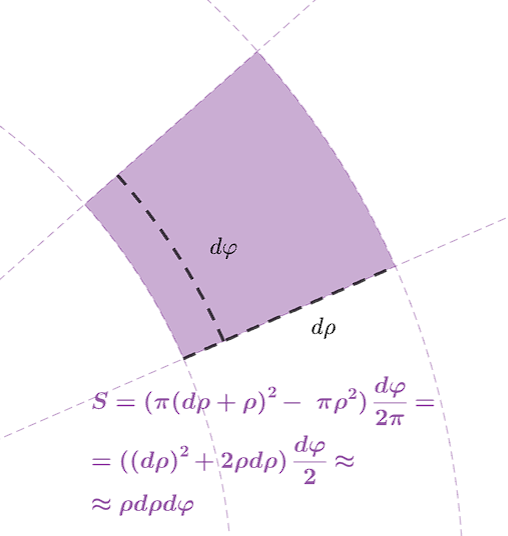
\includegraphics[height=7cm]{calculus/images/calculus_2024_04_10_2}
    \end{multicols}

    Заменим криволинейный параллелограмм $ABCD$ на обычный, стянув вершины хордами (погрешность в площади -- бесконечно малая более высокого порядка, чем площадь)

    $A = (x_A, y_A) = (\varphi(u, v), \psi(u, v))$

    $B = (x_B, y_B) = (\varphi(u, v+\Delta v), \psi(u, v+\Delta v))$

    $C = (x_C, y_C) = (\varphi(u + \Delta u, v+\Delta v), \psi(u + \Delta u, v+\Delta v))$

    $D = (x_D, y_D) = (\varphi(u + \Delta u, v), \psi(u + \Delta u, v))$

    Площадь параллелограмма $S_{ABCD} = AB \cdot AD \cdot \sin \theta = |\overrightarrow{AB} \times \overrightarrow{AD}|$

    $\Delta s = S_{ABCD} = |\overrightarrow{AB} \times \overrightarrow{AD}| = \left|
    \begin{vmatrix}
        \vec\imath & \vec\jmath & \vec{k} \\
        x_B - x_A          & y_B - y_A          & 0                  \\
        x_D - x_A          & y_D - y_A          & 0
    \end{vmatrix}\right| = \left| \vec{k}
    \begin{vmatrix}
        x_B - x_A & y_B - y_A \\
        x_D - x_A & y_D - y_A
    \end{vmatrix}\right|$

    $x_B - x_A = \varphi(u, v + \Delta v) - \varphi(u, v) = \Delta_v \varphi \approx \frac{\partial \varphi}{\partial v}\Delta v$

    $y_B - y_A = \psi(u, v + \Delta v) - \psi(u, v) = \Delta_v \psi \approx \frac{\partial \psi}{\partial v}\Delta v$

    $x_D - x_A = \varphi(u + \Delta u, v) - \varphi(u, v) = \Delta_u \varphi \approx \frac{\partial \varphi}{\partial u}\Delta u$

    $y_D - y_A = \psi(u + \Delta u, v) - \psi(u, v) = \Delta_u \psi \approx \frac{\partial \psi}{\partial u}\Delta u$

    $\left| \vec{k}
    \begin{vmatrix}
        x_B - x_A & y_B - y_A \\
        x_D - x_A & y_D - y_A
    \end{vmatrix}\right| = \left|
    \begin{vmatrix}
        \frac{\partial \varphi}{\partial v}\Delta v & \frac{\partial \psi}{\partial v}\Delta v \\
        \frac{\partial \varphi}{\partial u}\Delta u & \frac{\partial \psi}{\partial u}\Delta u
    \end{vmatrix}\right| = \left|
    \begin{vmatrix}
        \frac{\partial \varphi}{\partial u} & \frac{\partial \varphi}{\partial u} \\
        \frac{\partial \psi}{\partial v}    & \frac{\partial \psi}{\partial u}
    \end{vmatrix}\right| \stackrel{\Delta s^\prime}{\overgroup{\Delta v \Delta u}} \stackrel{|\det| = |J|}{\Longrightarrow} \Delta s \approx |J|\Delta s^\prime$

    \Nota В пределе это точное равенство: $|J| = \lim_{\Delta x \to 0} \frac{\Delta s}{\Delta s^\prime}$

    Это легко понять, если считать частные приращения по теореме Лагранжа $\Delta_u \varphi = \frac{\partial \varphi}{\partial u}(\xi, \eta) \Delta u \rightarrow \frac{\partial \varphi}{\partial u}(u, v) \Delta u$

    \hypertarget{determinantJaсobi}{}

    \Def Определитель $J = \begin{vmatrix}
        \frac{\partial x_1}{\partial \xi_1} & \dots  & \frac{\partial x_1}{\partial \xi_n} \\
        \vdots & \ddots & \vdots \\
        \frac{\partial x_n}{\partial \xi_1} & \dots  & \frac{\partial x_n}{\partial \xi_n} \\
    \end{vmatrix}$, где $\begin{cases}
                             x_1 = f_1(\xi_1, \dots, \xi_n) \\
                             \dots \\
                             x_n = f_n(\xi_1, \dots, \xi_n) \\
    \end{cases}$ -- преобразование координат $Ox_i \to O\xi_i \ (f_k \in C^1_D)$, называется определителем Якоби или якобиан

    \vspace{5mm}

    \textbf{Построение интеграла:}
    \begin{enumerate}
        \item Дробление $D^\prime$ в распрямленной $Ouv$
        \item Выбор средней точки, поиск значения $f(\xi_i, \eta_i)$

        Значение величины на элементе $f(\xi_i, \eta_i) |J| du dv$
        \item Интегральная сумма $\sigma_n = \sum f(\xi_i, \eta_i) |J| du dv$
        \item В пределе интеграл $\iint_D f(x, y) dx dy = \iint_{D^\prime} f(u, v) |J| du dv$
    \end{enumerate}

    \vspace{5mm}

    \textbf{Якобианы в ПСК, ЦСК, СфСК}

    \begin{enumerate}
        \item ПСК: $\quad \begin{cases}
                              x = \rho\cos\varphi \\ y = \rho\sin\varphi
        \end{cases} \quad
        \begin{matrix}
            \frac{\partial x}{\partial \rho} = \cos\varphi & \frac{\partial x}{\partial \varphi} = -\rho\sin\varphi \\
            \frac{\partial y}{\partial \rho} = \sin\varphi & \frac{\partial y}{\partial \varphi} = \rho\cos\varphi
        \end{matrix}$

        $J = \begin{vmatrix}\cos\varphi & -\rho\sin\varphi \\ \sin\varphi & \rho\cos\varphi\end{vmatrix} =
        \rho \begin{vmatrix}\cos\varphi & -\sin\varphi \\ \sin\varphi & \cos\varphi\end{vmatrix} = \rho$

        \item ЦСК: $\quad \begin{cases}
            x = \rho\cos\varphi \\ y = \rho\sin\varphi \\ z = z
        \end{cases} \quad J = \begin{vmatrix}\cos\varphi & -\rho\sin\varphi & 0 \\ \sin\varphi & \rho\cos\varphi & 0 \\ 0 & 0 & 1\end{vmatrix} = \rho$

        \item СфСК: $\quad \begin{cases}
            x = \rho\cos\varphi\sin\theta \\ y = \rho\sin\varphi\sin\theta \\ z = \rho \cos\theta
        \end{cases} \quad J = \begin{vmatrix}\cos\varphi\sin\theta & -\rho\sin\varphi\sin\theta & \rho\cos\varphi\cos\theta \\ \sin\varphi\sin\theta & \rho\cos\varphi\sin\theta & \rho\sin\varphi\cos\theta \\ \cos\theta & 0 & -\rho\sin\theta\end{vmatrix} = -\rho^2 \cos^2 \varphi \sin^3 \theta + \rho \sin \varphi \sin \theta (-\rho \sin \varphi \sin^2 \theta - \rho \sin \varphi \cos^2 \theta) - \rho^2 \cos^2 \varphi \cos^2 \theta \sin \theta = -\rho^2 (\cos^2 \varphi \sin \theta + \sin^2 \varphi \sin\theta) = -\rho^2 \sin \theta$

        $|J| = \rho^2 \sin \theta$
    \end{enumerate}

    \Ex Тело $T$, ограниченное уравнениями $\begin{matrix}x^2 + y^2 = z^2 \\ x^2 + y^2 = z\end{matrix}$

    Конус в ЦСК: $\rho = z, z > 0$

    Параболоид в ЦСК: $\rho = \sqrt{z}, z > 0$

    $V_T = \iiint_T dxdydz = \iiint_{T^\prime}\rho d\rho d\varphi dz = \int_0^{2\pi} d\varphi \int_0^1 d \rho \int_{z_1 = \rho^2}^{z_2=\rho} \rho dz =
    2\pi \int_0^1 \rho z \Big|_{z_1 = \rho^2}^{z_2=\rho} d\rho = 2\pi \int_0^1 (\rho^2 - \rho^3) d\rho =
    2\pi \left(\frac{\rho^3}{3} - \frac{\rho^4}{4}\right) \Big|_0^1 = 2\pi \left(\frac{1}{3} - \frac{1}{4}\right) = \frac{\pi}{6}$

    \Lab Тело $T$, ограниченное уравнениями $\begin{matrix}x^2 + y^2 + z^2 = 1 \\ \sqrt{x^2 + y^2} = z\end{matrix}$ -- \enquote{мороженка}, считать в СфСК


    \subsection{5.5. Криволинейные интегралы}

    \hypertarget{curvilinearintegraloffirstkind}{}

    Для криволинейных интегралов I рода область интегрирования -- кривая $l = \stackrel{\HUGE\frown}{AB}$ (дуга). Для простоты начнем с плоской дуги

    На $l$ действует скалярная функция $f(x, y)$ (физический смысл -- плотность, то есть имеем неоднородный кривой стержень)

    Задача в нахождении \enquote{суммарной} величины $f(x, y)$, то есть интеграла: \enquote{складываем} элементы $f_{\text{ср}}(x, y) dl$

    Получаем $\int_l f(x, y)dl = \int_{AB} f(x, y)dl$
\end{document}



